\documentclass[11pt,a4paper]{article}
\usepackage[T1]{fontenc}
\usepackage[utf8]{inputenc}
\usepackage{lmodern}
\usepackage[margin=2.2cm]{geometry}
\usepackage{booktabs}
\usepackage{tabularx}
\usepackage{array}
\usepackage{enumitem}
\usepackage{caption}
\usepackage{float}
\usepackage{tikz}
\usetikzlibrary{positioning,arrows.meta,fit}
\usepackage[hidelinks]{hyperref}

\setlist{nosep,leftmargin=*}
\captionsetup{font=small,labelfont=bf}
\renewcommand{\arraystretch}{1.2}
\newcolumntype{R}{>{\raggedleft\arraybackslash}p{1.35cm}}

\title{\textbf{Distill}: Keep the Knowledge, Lose the Weight\\[4pt]
\large Ericsson Build Hackathon 2026 --- Data Storage Optimization}
\author{Team Distill}
\date{14 November 2026}

\begin{document}
\maketitle

\begin{abstract}
Distill reduces the storage used by Ericsson's recordings and documents without losing the information inside them.
Videos are turned into slide pictures, a speaker-attributed transcript and short voice samples; official documents are kept as originals,
copies become references and older revisions are stored as their changes only.
On Ericsson's 12 sample files, total storage fell from \textbf{1.45\,GB to 25.0\,MB (98.3\%)}.
Everything runs offline on a laptop CPU.
\end{abstract}

%======================================================================
\section{Architecture}

Distill scans three sources, fingerprints every file, and processes videos and documents in two pipelines.
Results are stored in an SQLite database and a content-addressed object store (each picture stored once).
A FastAPI backend serves them to a Next.js user interface.

\begin{figure}[H]
\centering
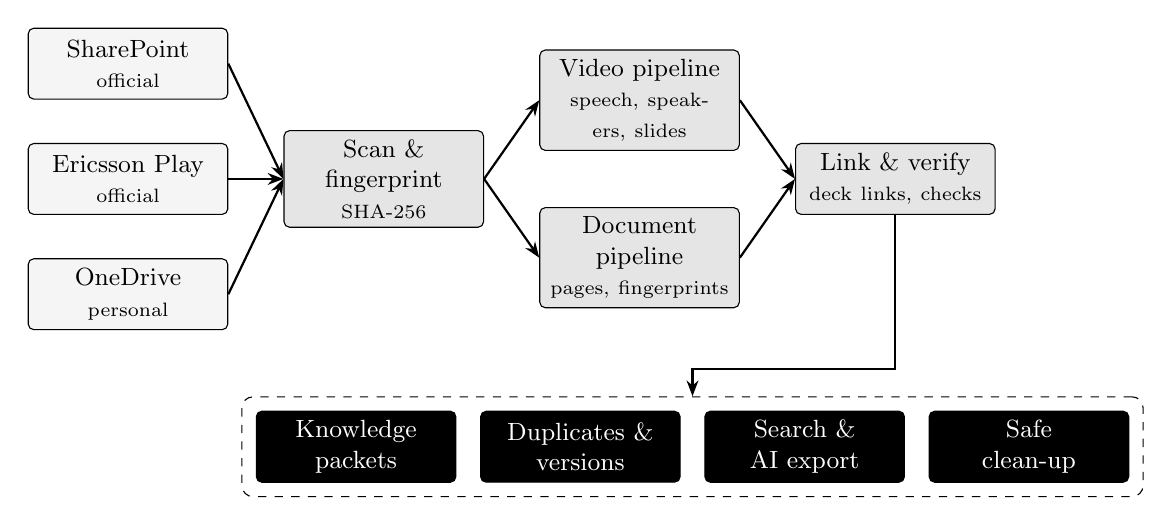
\begin{tikzpicture}[
  node distance=0.55cm and 0.6cm,
  box/.style={draw, rounded corners=2pt, minimum height=0.9cm, align=center, font=\small, text width=2.3cm},
  src/.style={box, fill=gray!8},
  proc/.style={box, fill=gray!20},
  outbox/.style={box, fill=black, text=white, text width=2.3cm},
  arr/.style={-{Stealth[length=2mm]}, thick}]
  \node[src] (sp) {SharePoint\\\scriptsize official};
  \node[src, below=of sp] (play) {Ericsson Play\\\scriptsize official};
  \node[src, below=of play] (od) {OneDrive\\\scriptsize personal};
  \node[proc, right=0.7cm of play] (scan) {Scan \&\\fingerprint\\\scriptsize SHA-256};
  \node[proc, right=0.7cm of scan, yshift=1.0cm] (vid) {Video pipeline\\\scriptsize speech, speakers, slides};
  \node[proc, right=0.7cm of scan, yshift=-1.0cm] (doc) {Document pipeline\\\scriptsize pages, fingerprints};
  \node[proc, right=0.7cm of vid, yshift=-1.0cm] (link) {Link \& verify\\\scriptsize deck links, checks};
  \draw[arr] (sp.east) -- (scan.west);
  \draw[arr] (play.east) -- (scan.west);
  \draw[arr] (od.east) -- (scan.west);
  \draw[arr] (scan.east) -- (vid.west);
  \draw[arr] (scan.east) -- (doc.west);
  \draw[arr] (vid.east) -- (link.west);
  \draw[arr] (doc.east) -- (link.west);
  \node[outbox, below=1.3cm of doc, xshift=-3.6cm] (o1) {Knowledge\\packets};
  \node[outbox, right=0.3cm of o1] (o2) {Duplicates \&\\versions};
  \node[outbox, right=0.3cm of o2] (o3) {Search \&\\AI export};
  \node[outbox, right=0.3cm of o3] (o4) {Safe\\clean-up};
  \node[draw, dashed, rounded corners, fit=(o1)(o2)(o3)(o4), inner sep=5pt] (outs) {};
  \draw[arr] (link.south) |- ([yshift=0.35cm]outs.north) -- (outs.north);
\end{tikzpicture}
\caption{Distill architecture. Official sources are SharePoint and Ericsson Play; OneDrive is a personal drive.}
\end{figure}

%======================================================================
\newpage
\section{Tools and models}

Only four AI models are used; everything else is a deterministic algorithm. All run offline.

\begin{table}[H]
\centering
\small
\begin{tabularx}{\textwidth}{@{}l l X@{}}
\toprule
\textbf{Tool} & \textbf{Type} & \textbf{Used for} \\
\midrule
Whisper base (faster-whisper, int8) & AI model & Speech to text with word timestamps \\
pyannote 3.0 + WeSpeaker (sherpa-onnx) & AI model & Who spoke when (speaker detection) \\
RapidOCR (PaddleOCR, ONNX) & AI model & Reading text on slide pictures and PNG images \\
all-MiniLM-L6-v2 & AI model & Search by meaning \\
FFmpeg, OpenCV & Algorithm & Reading video, audio extraction, slide-change detection \\
Opus (16\,kbps), WebP (q70), gzip & Algorithm & Compressing audio, pictures and text \\
SHA-256 & Algorithm & Exact fingerprints of files and slide texts \\
pHash / dHash & Algorithm & Picture fingerprints (look-alike slides, duplicate videos) \\
PyMuPDF, python-pptx, LibreOffice & Library & Reading and rendering PDF and PowerPoint pages \\
olefile, XML parsing & Library & Reading e-mails (MSG) and Word files (DOCX) \\
SQLite + FTS5 & Database & Storage and keyword search \\
FastAPI, Next.js & Web & Backend API and user interface \\
\bottomrule
\end{tabularx}
\caption{Tools and models.}
\end{table}

%======================================================================
\section{How each file type is compressed}

\subsection{Videos}
\begin{enumerate}
  \item \textbf{Fingerprint} the original (SHA-256) so it can later be proven unchanged.
  \item \textbf{Extract audio} (FFmpeg) and \textbf{transcribe} it (Whisper): every sentence with start and end time.
  \item \textbf{Detect speakers} (pyannote + WeSpeaker) and keep an 8-second voice sample per speaker.
  \item \textbf{Detect slide changes} (OpenCV), ignoring the webcam area; keep one picture per slide, taken just before it changes.
  \item \textbf{Read each slide} (RapidOCR) and \textbf{link} it to the official deck page (75\% word overlap + 25\% picture similarity, threshold 55\%).
  \item \textbf{Package} the result: Opus audio, WebP slide pictures, gzipped transcript and notes.
\end{enumerate}

The package can be stored at five levels. Each level is the sum of the files it keeps:

\begin{table}[H]
\centering
\small
\begin{tabularx}{\textwidth}{@{}l X R R R@{}}
\toprule
\textbf{Level} & \textbf{What is kept} & \textbf{Meeting} & \textbf{GraalVM} & \textbf{Jury} \\
\midrule
1 Original & Full video & 1166.39 & 210.27 & 84.55 \\
2 Smaller video & Re-encoded: H.264, 5\,fps, max 1280\,px & 157.75$^{*}$ & 5.70 & 13.84 \\
3 Audio + slides + text & Opus audio + slide pictures + transcript + voices & 24.07 & 2.21 & 1.44 \\
\textbf{4 Slides + text} & \textbf{Level 3 without the audio (default)} & \textbf{7.47} & \textbf{0.62} & \textbf{0.94} \\
5 Text + links & Level 4; linked slides replaced by links to the deck & 5.49 & 0.62 & 0.94 \\
\bottomrule
\end{tabularx}
\caption{Size per level in MB (1\,MB = 1024\,KB). $^{*}$Estimated: Level 2 is not created for videos longer than 25 minutes.}
\end{table}

\subsection{PDF and PowerPoint}
Every page is read directly from the file (PyMuPDF, python-pptx) and drawn as a picture (LibreOffice for PowerPoint).
Each page gets a text fingerprint (SHA-256 of the cleaned text, footers and page numbers removed) and a picture fingerprint (pHash).
Revisions are read from Ericsson's document control, e.g.\ \texttt{Uen | A | 2019-10-11}. Storage policy:
\begin{itemize}
  \item \textbf{Official copy:} the original file is kept unchanged.
  \item \textbf{Exact copy elsewhere:} replaced by a reference to the official copy (0\,B).
  \item \textbf{Older revision:} only the slides that differ from the newest revision are stored, plus references to the shared slides.
\end{itemize}

\subsection{Word, e-mail and image files}
Word (DOCX) and e-mail (MSG) text is extracted for search; the official Word file is kept, the e-mail is stored as compressed text.
Images (PNG) are fingerprinted with SHA-256 and their text is read with OCR; an exact copy becomes a reference.

%======================================================================
\section{Results per file}

\begin{table}[H]
\centering
\footnotesize
\begin{tabularx}{\textwidth}{@{}r X l r r r l@{}}
\toprule
\# & \textbf{File} & \textbf{Source} & \textbf{Initial MB} & \textbf{Final MB} & \textbf{Saved} & \textbf{Stored as} \\
\midrule
1 & Brief.png & SharePoint & 0.22 & 0.22 & 0.0\% & Original \\
2 & C2L Presentation (Rev B).pdf & SharePoint & 3.38 & 3.38 & 0.0\% & Original \\
3 & Challenge\_Ericsson.docx & SharePoint & 0.27 & 0.27 & 0.0\% & Original \\
4 & Ericsson Response Intro.pdf & SharePoint & 8.37 & 8.37 & 0.0\% & Original \\
5 & SD-WAN final.pptx (Rev B) & SharePoint & 3.51 & 3.51 & 0.0\% & Original \\
6 & Meeting recording (155 min) & SharePoint & 1166.39 & 7.47 & 99.4\% & Slides + text \\
7 & GraalVM talk (16 min) & Ericsson Play & 210.27 & 0.62 & 99.7\% & Slides + text \\
8 & Jury and prizes (6 min) & Ericsson Play & 84.55 & 0.94 & 98.9\% & Slides + text \\
9 & C2L Presentation (Rev B) (1).pdf & OneDrive & 3.38 & 0.00 & 100.0\% & Reference \\
10 & Copy of Brief.png & OneDrive & 0.22 & 0.00 & 100.0\% & Reference \\
11 & SD-WAN final2.pptx (Rev A) & OneDrive & 3.30 & 0.20 & 94.0\% & Delta (7 + 18 ref.) \\
12 & Chat history.msg & OneDrive & 0.08 & 0.00 & 99.2\% & Text \\
\midrule
 & \textbf{Total} & & \textbf{1483.94} & \textbf{24.99} & \textbf{98.3\%} & \\
\bottomrule
\end{tabularx}
\caption{Initial and final size per file (1\,MB = 1024\,KB). A final size of 0.00 is a reference of a few bytes; file 12 is 656 bytes. Delta = 7 changed slides stored + 18 references to Rev B.}
\end{table}

Quality checks on the meeting recording: 95.8\% of on-screen slide text is found in the kept slides,
90\% of checked moments match by direct picture comparison, and OCR reads 95.1\% of the words of 36 official slides correctly.
The original files are never changed (verified with SHA-256).

\end{document}
